\documentclass{phyasgn}\usepackage{nag}
\phyasgn{classname=宽禁带半导体课程论文}
\usepackage[backend=bibtex,bibstyle=gb7714-2015,citestyle=gb7714-2015]{biblatex}
\setlength{\bibitemsep}{3bp}
\addbibresource{ref.bib}
\renewcommand*{\bibfont}{\zihao{5}\linespread{1.27}\selectfont}
\usepackage{background}
\usepackage{siunitx}
\backgroundsetup{scale=1,angle=0,opacity=1,contents={
\includegraphics[width=\paperwidth, height=\paperwidth, keepaspectratio]{pic/phy.jpg}}}
%\ctexset{punct=kaiming}
\setCJKmainfont[ItalicFont=FZKTK.TTF,BoldFont=FZXBSK.TTF]{FZSSK.TTF}
\setCJKsansfont[BoldFont=FZHTK.TTF]{FZXH1K.TTF}
\setCJKmonofont[ItalicFont=FZKTK.TTF]{FZFSK.TTF}
\newCJKfontfamily\FZSS{FZSSK.TTF}
\newCJKfontfamily\FZKT{FZKTK.TTF}
\newCJKfontfamily\FZFS{FZFSK.TTF}
\newCJKfontfamily\FZHT{FZHTK.TTF}
\setmainfont{TeX Gyre Termes}
\setsansfont{TeX Gyre Heros}[Scale=MatchLowercase]
\setmonofont{Ubuntu Mono}%[Scale=MatchLowercase]
\newfontfamily\lm{Latin Modern Roman}
\usepackage{unicode-math}
\setmathfont{TeX Gyre Termes Math}

\newcommand\pkg[1]{\textsf{#1}}
\newenvironment{csop}{\vskip\topsep\noindent\hspace{2em}\ttfamily\small\ignorespaces}{\vskip\topsep\par}
\usepackage{float}
\usepackage{booktabs,metalogo,siunitx,marginnote,manfnt,url}
\usepackage[unicode]{hyperref}
\hypersetup{pdfstartview=XYZ,hidelinks,pdfcreator=XeTeX Output,pdfauthor=吴熙楠,
pdftitle=钙钛矿发光材料}
\usepackage{geometry,fancyhdr}
\geometry{left=3cm,right=3cm,marginparwidth=4em}
\fancyhead[L]
{\begin{tabular}[b]{@{}l@{}}
  \hyperref{https://www.phy.pku.edu.cn/}{}{}{
\includegraphics[height=2.12em]{phylogo.pdf}}
\end{tabular}}
\fancyhead[C]
{\begin{tabular}[b]{@{}c@{}}
  \large 
  钙钛矿发光材料
  \\[-2pt]
  {\scriptsize 姓名:~吴熙楠\quad 学号:~1900011413}
\end{tabular}
}

\usepackage{shortvrb,fancyvrb}
\MakeShortVerb|
\fvset{xleftmargin=2em,fontsize=\small}
\makeatletter
\ifx\l@nohyphenation\undefined
  \newlanguage\l@nohyphenation
\fi
\DeclareRobustCommand\meta[1]{%
  \ensuremath\langle
  \ifmmode \expandafter \nfss@text \fi
  {%
    \rmfamily\itshape
    \edef\meta@hyphen@restore
    {\hyphenchar\the\font\the\hyphenchar\font}%
  \hyphenchar\font\m@ne
  \language\l@nohyphenation
  #1\/%
  \meta@hyphen@restore
  }\ensuremath\rangle
}
\makeatother

\def\phyasgn{\pkg{phyasgn}}
\def\version{0.2 $\upbeta$}

\title{
  {钙钛矿发光材料}\\[-8pt]
    {\normalsize ——宽禁带半导体课程论文}
}
\author{吴熙楠}
\date{\today}

\begin{document}
\maketitle
\begin{abstract}
金属卤化物钙钛矿作为新一代半导体材料,已广泛应用于各种光电器件,尤其是钙钛矿发光二极管领域。在过去的几年里,绿色、红色和近红外PeLED的外部量子效率已经超过25\%,与有机发光二极管(OLED)和量子点发光二极管(QLED)相当。然而蓝光PeLED的性能远远落后于它们的对应产品,这是由于蓝钙钛矿薄膜的低量子产率,发射光谱的不稳定性,以及电荷注入的困难。本文首先介绍了钙钛矿材料的基本性质和PeLED的结构特点,并将其与OLED和QLED进行一些对比,接着提出了蓝光发射PeLED目前面临的一些困难,最后对一些提高蓝光发射的PeLED效率的方法进行了讨论并展望未来PeLED的发展。
\end{abstract}
\tableofcontents
\section{引言}
在发光器件的发展史上,按时间顺序出现的最常用的电灯是白炽灯、荧光灯和发光二极管。与白炽灯/荧光灯相比,LED有很多优势,具有更少的能源消耗和纳秒响应速度。除了在照明领域的应用,LED还因其发光效率高、发射光谱窄、颜色可调、稳定性好等优点被广泛应用于高清显示器。目前,发光半导体材料主要包括金属配合物、有机小分子和聚合物、量子点、金属卤化物钙钛矿等。
\par 金属卤化物钙钛矿(MHP)具有特殊的光电子特性,包括高光致发光量子子产率、低陷阱态密度、高颜色纯度和宽色域。作为一种新兴的半导体材料,MHP近年来受到了广泛研究,并已成功应用于一系列光电器件,如太阳能电池、LED、光电探测器和新型激光器等。2014年,Friend的团队首次展示了在室温下工作的电致发光PeLED,其中近红外(754nm)和绿光(517nm)PeLED的外量子效率分别为0.76\%和0.1\%。近年来,绿光、红光和近红外PeLED的EQE均超过25\%,与有机发光二极管(OLED)和量子点发光二极管(QLED)的EQE相当。然而,蓝光PeLED的效率提高仍然停滞不前,特别是真正的蓝光PeLED。目前,发射波长在455-470nm之间的蓝光PeLED的最高EQE小于6\%。图1中对2014年以来红、绿、蓝三种颜色的PeLED的发展趋势进行了说明和比较。
\begin{figure}[H]
	\centering
	\hspace{2em}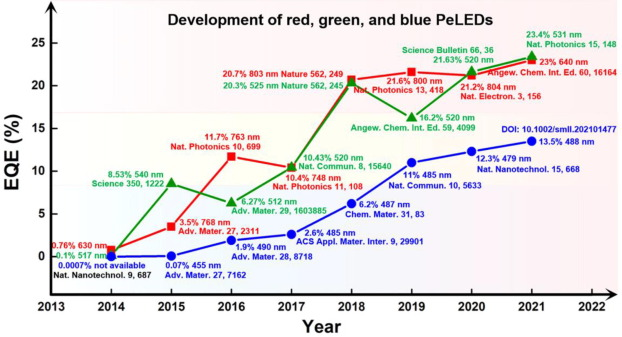
\includegraphics[width=.8\linewidth]{pic/5.jpg}
	\caption{2014年以来PeLED的发展趋势及成果\cite{zhang2021blue}
	}
\end{figure}
\par 蓝光发射是三基色最重要的组成部分之一,是固态照明和显示器的必要组成部分,但蓝光LED的效率进展总是远远落后于绿色和红色发光二极管,主要原因是在制备高质量的蓝色发光层和注入载流子方面存在困难,以及它们的运行稳定性较差。目前,蓝光PeLED的开发存在许多障碍,阻碍了其性能的提高和商业应用。例如,合成钙钛矿时形成的Cl空位在带隙内形成深阱态,导致严重的非辐射复合。此外,具有卤素空位的混合卤化物钙钛矿在光场和电场作用下表现出严重的离子迁移,容易偏析成富Cl和富Br相,这导致了不稳定的发射光谱。而且对于蓝色发射的胶体钙钛矿纳米片或胶体钙钛矿量子点(PeQD),其旋涂的薄膜的导电性相对较差,这是因为包裹在纳米颗粒表面的绝缘有机配体大大降低了载体的注入和输运率,从而降低了辐射复合效率。因此,目前看来PeLED还需要进一步的发展解决这些问题才能达到商用化的地步。。
\par 在这篇课程论文中,我们首先介绍了钙钛矿材料的基本性质和PeLED的结构特点,并将其与OLED和QLED进行一些对比,接着提出了蓝光发射PeLED目前面临的一些困难,最后对一些提高蓝光发射的PeLED效率的方法进行了讨论并展望未来PeLED的发展。
\section{金属卤化物钙钛矿(MHP)材料}
\begin{figure}[H]
	\centering
	\hspace{2em}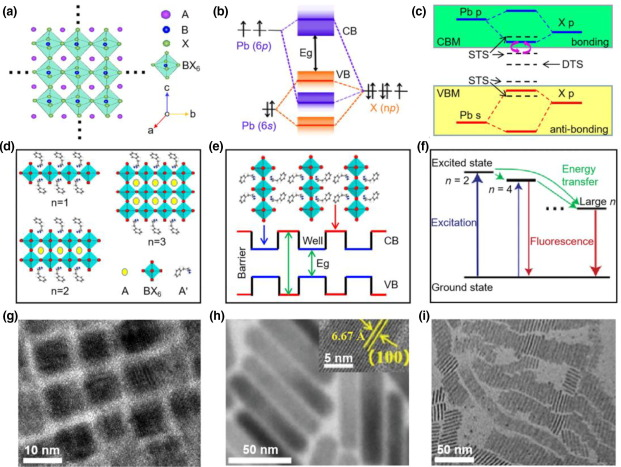
\includegraphics[width=.8\linewidth]{pic/1.jpg}
	\caption{(a)3D钙钛矿的晶体结构;(b)3D钙钛矿能带轨道示意图;(c)浅能级和深能级的形成过程;(d) 2D 钙钛矿的结构;(e)2D钙钛矿的多个量子阱结构;(f)准2D钙钛矿中的级联能量转移示意图;(g) CsPb(Cl/Br)$_3$ PeQD在170\si{\degreeCelsius}下合成的透射电镜图像;(h) 1D CsPb$_{0.08}$Cd$_{0.92}$Br$_3$纳米棒示意图;(i) CsPbBr$_3$纳米棒在180\si{\degreeCelsius}加热20min后示意图。\cite{zhang2021blue}
	}
\end{figure}
	\begin{figure}[H]
		\centering
		\hspace{2em}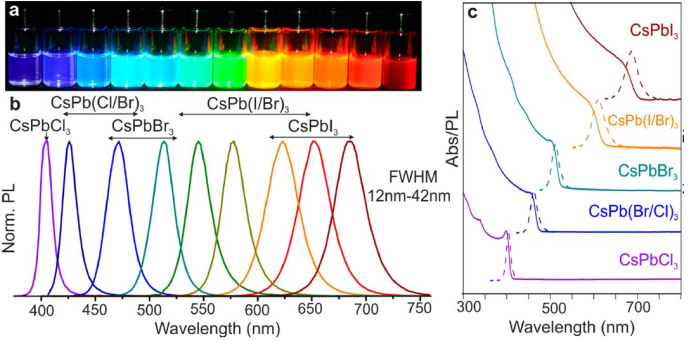
\includegraphics[width=.8\linewidth]{pic/2.png}
		\caption{CsPbX$_{3}$钙钛矿组分调控实现光谱调控\cite{yakunin2015low}
		}
	\end{figure}
\subsection{3D 钙钛矿}
\par MHP的典型晶体结构与天然矿物钙钛氧化物(CaTiO$_3$)相同,CaTiO$_3$是由德国矿物学家Gustav Rose 于1839年发现的,并以LevPerovski的名字命名。MHP呈现三维结构,一般化学式为ABX$_3$,其中A位被一价阳离子(如MA$^+$,FA$^+$或Cs$^+$)占据;B位是二价金属阳离子(如Pb$^{2+}$或Sn$^{2+}$);X位是卤素离子(如I$^{-}$,Br$^{-}$或Cl$^{-}$),六个X位卤素离子形成一个八面体,中间有一个二价的B位金属阳离子。这样一系列角共享八面体无限延伸,形成一个三维网络,A位阳离子占据八个相邻角共享八面体之间的空腔,保持系统的电中性(图2a)。将A、B和X离子分别用离子半径R$_{A}$、R$_{B}$和R$_{X}$作为刚性球体处理,其容错因子定义为$t=\dfrac{R_{A}+R_{X}}{\sqrt{2}(R_{B}+R_{X})}$,典型的3D钙钛矿结构$0.78\le t\le 1.05$。
\par 通过二价B位阳离子、卤素离子的交替,可以调节MHP的带隙(图2b),因此,使用不同或混合的卤素离子来控制MHP的发射波长是最广泛采用的方法,通过改变X离子的比例\footnote{ CsPbI$_{3}$的禁带宽度是$1.73eV$\cite{swarnkar2016quantum},CsPbBr$_{3}$的禁带宽度是$2.35 eV$\cite{becker2018bright}, CsPbCl$_{3}$ 的禁带宽度是 $3.06 eV$\cite{becker2018bright}。},钙钛矿发光材料的PL光谱可以在$400-800 nm$ 的范围内连续可调,覆盖了整个可见光区域\cite{stranks2015metal}。不过A,M,X三种离子的混合对钙钛矿的能带结构都有一定影响,从而会导致在加入外场或者光生载流子时发光峰位的移动\cite{sutherland2016perovskite}。
\par 由于无机CsPbX$_3$(X=Cl,Br或I)钙钛矿的软晶格结构和低形成能(从上述的典型3D钙钛矿的容错因子也可以看出),卤素空位是其主要的缺陷态\cite{pan2019halogen}。CsPbBr$_3$和CsPbI$_3$钙钛矿的缺陷态分别由Br空位和I空位引起,是浅陷阱态。在热激活下,被这些浅层陷阱捕获的载流子可以返回到带边缘,然后辐射重组。而CsPbCl$_3$钙钛矿中的Cl空位在带隙中以高度局域化的陷阱态存在,这会导致其缺陷态有效捕获电荷和显著的非辐射重组,从而导致Cl基钙钛矿的低缺陷容错性特征,因此,Cl空位的钝化是含Cl混合卤化物钙钛矿的重要课题。
\subsection{钙钛矿量子点(PeQD)}
零维(0D)胶体钙钛矿纳米晶体,也被称为钙钛矿量子点(PeQD),在发光特性上有着接近100\%的PLQY。胶体量子点在三个垂直方向上的生长受到表面有机配体(如油酸和油胺)的限制。
\par 钙钛矿量子点由于量子限域效应,激子束缚能较大,同时俄歇复合常数较小,因此在得到较好的表面钝化过后会量子产率非常高,接近100\%\cite{li2016cspbx3}(其余荧光LED材料在激发浓度较小时PLQY会明显下降)。目前有多种合成钙钛矿胶体量子点的方法,如常规热注入法、室温配体辅助再沉淀法、超声合成法等。热注入法和配体辅助再沉淀法都可以通过卤化物组成来合成不同的量子点,其平均粒子直径小于玻尔直径。
\section{钙钛矿发光二极管(PeLED)}
\subsection{PeLED的基本构成}
	\begin{figure}[H]
		\centering
		\hspace{2em}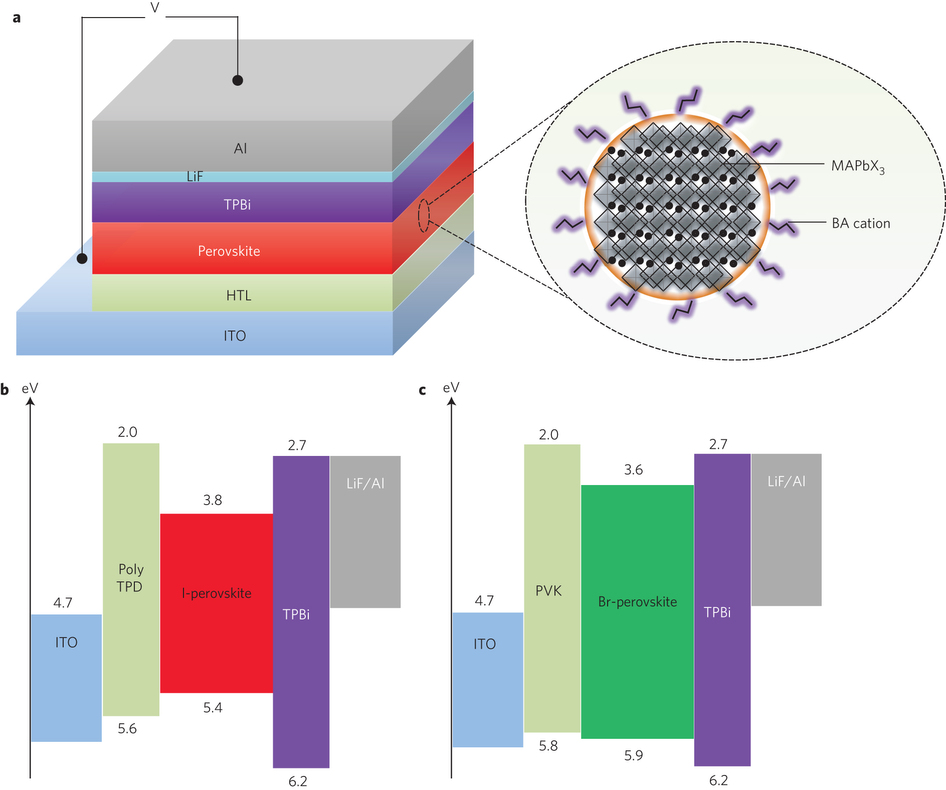
\includegraphics[width=.7\linewidth]{pic/6.jpg}
		\caption{钙钛矿发光二极管结构图及能量图
		}
	\end{figure}
\par  一个完整的PeLED器件至少有以下五个功能层组成(如图4),依次包括阴极、电子传输层、钙钛矿发光层、空穴传输层和阳极。阴极材料负责向电子传输层注电子,一般以低功函数的材料,如Ca,Al,Ag等金属较为多见。电子传输层将阴极注入的电子传输并注入到发光层,要求电子迁移率高,导带 位置合适,常见的有ZnO,TiO$_{2}$等氧化物纳米晶或者部分小分子有机物材料。发光层为钙钛矿,注入的电子和空穴在此复合,因此要求荧光量子产率尽量高,同时价带导带能级位置合适以满足载流子平衡注入的要求。空穴传输层将阳极注入的空穴运输并注入到发光层,因此要求空穴迁移率高,价带位置合适,常见的有NiO及部分有机物材料。阳极负责向空穴传输层注入空穴,一般要求高功函数的材料,常见有铟锡氧化物透明导电薄膜(ITO),氟掺杂的SnO$_{2}$透明导电薄膜(FTO)和金属Au等。
\par 注入的电子和空穴在发光层中相遇,形成激子后发生辐射复合或电子和空穴作为自由载流子直接发生双分子复合最后复合产生的光子穿过各个功能层后射出器件。
\par 钙钛矿层的折射率一般比较大(如FAPbI$_{3}$折射率为2.7),且通常钙钛矿材料发光是各向同性的,因此,考虑到全反射条件的限制,将有很大一部分辐射出来的光子无法射出器件,但是这是在每层不增加光提取的情况下得出的结论,通过课程上学到的光子晶体的概念,我们可以设想在钙钛矿发光层表面制作周期性的光子晶体结构,这样由于光子晶体的倒格矢帮助下能够实现出光的衍射增强。但是由于钙钛矿发光层薄膜的制作比较特殊(在本文4.1节会提到),薄膜的形成与结晶与旋涂同步紧密相关,因此不能够先制作好材料再进行结构的设计,需要在旋涂过程中就进行好结构设计,不过如果是在本身具有结构的衬底上旋涂或者使用喷墨打印的方法或许能够实现。
\par PeLED器件的总厚度往往不超过300 nm,发光中心到金属电极的距离小于半波长。此时PeLED中将出现明显的近场光学效应,金属电极会带来强烈的表面等离子共振吸收,造成大量光损耗。这里上课老师提问金属电极带来的表面等离子激元共振吸收如何转换为光能增强出光效率方面,关键是有没有结构模式之间的耦合,通过查找相关文献可以找到表面等离子激元共振既可以产生热能损耗也有可能提高出光效率,如果将金属电极表面制作为周期性的阵列形式可能会利用LSP与SPP耦合来增强量子点出光效率与荧光稳定性\cite{rai2021engineering},不过目前这样的研究只存在于传统CdSe/ZnS量子点或者2D的WS$_2$纳米片体系,尚未查找到有关胶体钙钛矿量子点尤其是Cl基胶体钙钛矿量子点体系的研究,因此对于PeLED电极部分结构的设计可能也会成为未来的一个方向。
\par 钙钛矿消光系数很高($\sim$10$^{4}$cm$^{-1}$),在部分钙钛矿比较厚的PeLED器件中存在显著的自吸收现象,也可能会造成光子的消耗(不过这也能通过每层增加光提取结构来解决)\cite{cho2020role}。
\subsection{PeLED的特点}
\par PeLED的一个重要的特点是窄发光峰宽带来的高色纯度。作为一种直接带隙半导体材料,钙钛矿的荧光来自于带边自由载流子的直接复合(如三维钙钛矿,激子束缚能较小,基本不受到晶体尺寸的影响)或带边激子直接复合(钙钛矿量子点,激子束缚能较大的情况),因此钙钛矿的荧光半峰宽非常窄。
\par PeLED发光层的沉积过程伴随着钙钛矿的形成与结晶的过程,薄膜沉积工艺不但影响钙钛矿薄膜的形貌,也极大地影响着钙钛矿膜的发光性质(OLED与QLED都需要先合成发光材料,然后再蒸镀、旋涂、喷墨打印等方法沉积成发光层,沉积过程原则上只影响发光层的形貌而不会影响发光性质)。
\par PeLED的离子迁移问题:由于钙钛矿本质上是一种离子晶体,当有外加电场存在或者有光生载流子时,钙钛矿中的离子(主要是卤素离子)会从晶体结构比较“脆弱”的地方,如晶界、表面等存在大量缺陷的地方开始发生移动,从而导致器件性能的衰减\cite{wang2016stability}(解决方法暂时只有表面处理钝化)。
\par PeLED的迟滞现象:受到离子迁移的影响,PeLED的电流-亮度-电压曲线和效率-电压曲线在正扫和反扫是不重合的,等效于会造成器件功能的不稳定性(如图5)。
	\begin{figure}[H]
		\centering
		\hspace{2em}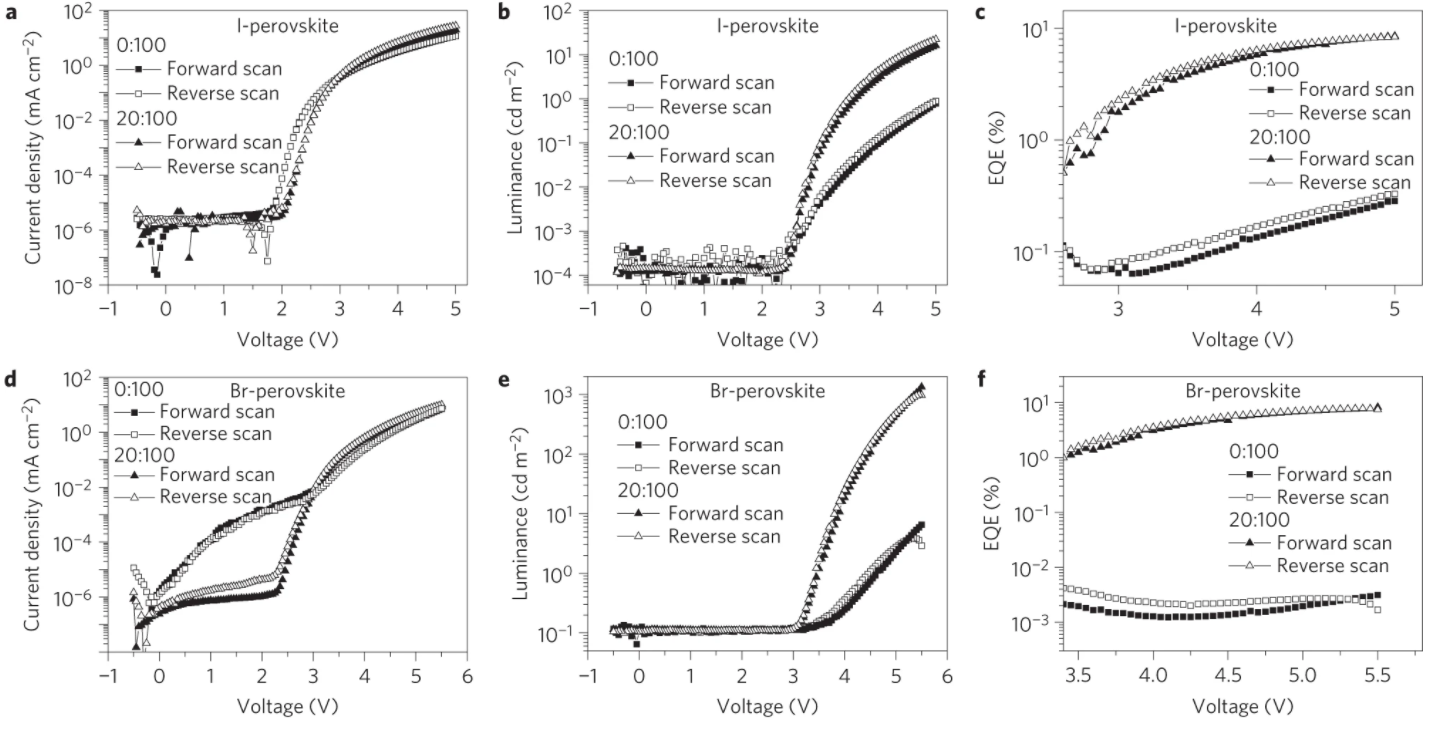
\includegraphics[width=.9\linewidth]{pic/4.png}
		\caption{迟滞效应对PeLED性能的影响\cite{xiao2017efficient}
		}
	\end{figure}
\subsection{PeLED与OLED和QLED的对比}
\begin{figure}[H]
	\centering
	\hspace{2em}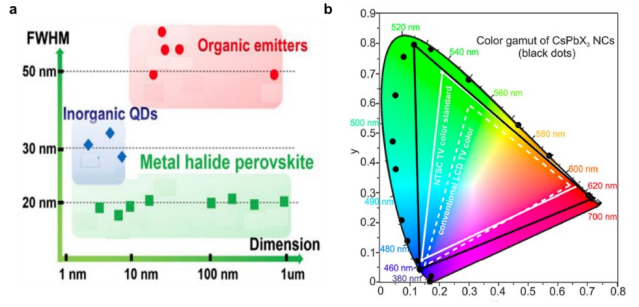
\includegraphics[width=.8\linewidth]{pic/3.png}
	\caption{a.钙钛矿、量子点、有机发光材料的半峰宽对比;b.钙钛矿发光材料色域覆盖范围\cite{yakunin2015low}
	}
\end{figure}
\par 光谱方面,PeLED和QLED都可以通过组分调节以及量子限域效应的方法改变发光峰位,电致荧光可以从整个可见光范围延伸到近红外区域。OLED要实现发光峰位的移动则需要合成不同的发光分子,光谱范围基本集中在可见光区域。同时钙钛矿材料的单线态与三线态能级差别很小,能实现快速转换,因此允许光学跃迁态\footnote{单线态电子自旋为0,跃迁前后自旋不变,三线态电子自旋可能会出现跃迁后的自旋反转现象,因此单线态为光学允许态。}(单线态)比例很高。
\par 色纯度方面,由于有机材料固有限制,OLED(FWHW>50 nm)比QLED(FWHW$\sim$30nm)和PeLED(FWHW<20nm)都要略逊一筹,因此PeLED在色纯度方面表现尤其出色,能够覆盖更广的色域空间,非常适合用于高性能显示器件。
\par 器件方面,OLED的最高效率往往在低亮度下达到,高电流高亮度情况下则伴随着显著的效率滚降,而QLED 和PeLED都报道了效率滚降很小的器件,满足了高亮度场景的使用要求。(OLED与QLED目前都已经有超过百万小时寿命的器件报道,OLED更是已经投入了商业化应用,而PeLED的稳定性研究才刚刚起步不久,报道的最佳寿命也仅仅数百小时\cite{wang2019trifluoroacetate}。)
\par 工艺方面,三种器件都可以通过低成本的低温溶液加工工艺生产制备,都可以兼容柔性衬底,而OLED除了溶液工艺之外还可以通过真空蒸镀的方式制备,对于OLED而言其制备流程已经非常完善了。
\clearpage
\section{蓝光PeLED}
\subsection{蓝光PeLED薄膜制备方法}
\begin{figure}[H]
		\centering
		\hspace{2em}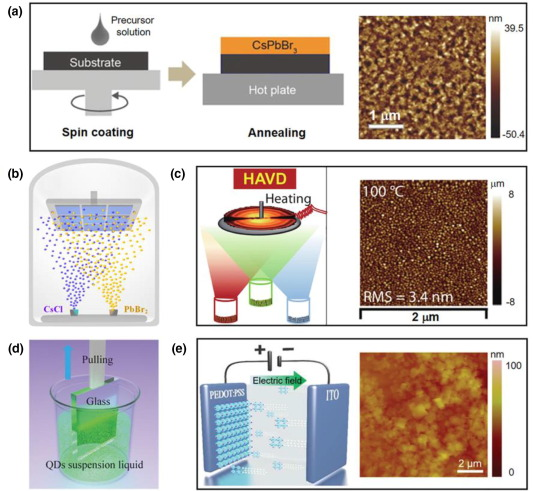
\includegraphics[width=.8\linewidth]{pic/7.jpg}
		\caption{(a)一步旋转镀膜的原理图(b)双源共蒸发示意图(c)加热辅助真空沉积示意图(d)浸涂法制备有机金属卤化物PeQD薄膜示意图(e)制备(PEA)$_{2}$PbBr$_{4}$薄膜过程示意图\cite{zhang2021blue}}
\end{figure}
\par 用于PeLED的3D钙钛矿多晶薄膜通常是由AX和BX$_2$在二甲基甲酰胺或二甲亚砜溶剂通过一步旋涂法溶解制备的钙钛矿前驱体溶液得到的(如图7a)。然而对于基于混合卤素(Cl和Br)钙钛矿的蓝色PeLED,由于卤化铯盐的溶解性差,结晶速度快,旋涂法制备的全无机钙钛矿CsPbBr$_x$Cl$_{3-x}$薄膜表面粗糙度大,膜层覆盖不完全,这样的不完全会导致严重的非辐射电流损失。为了解决这些问题,我们可以采用热蒸发法(如图7b),可以将两种卤化物混合制备了致密光滑的蓝光CsPbBr$_x$Cl$_{3-x}$。此外,目前也有一种加热辅助真空沉积的方法来制备全无机深蓝色发射型钙钛矿薄膜,在钙钛矿沉积过程中,将基片在预先设定的温度下加热。得到了致密、晶粒均匀、表面粗糙度低的全无机蓝钙钛矿膜(如图7c)。
\par 大多数Cs基胶体钙钛矿量子点制备的薄膜是通过一步旋转涂覆方法制备的,然而有机金属卤化物量子点合成PeQD悬浮液的浓度较低,因此我们利用稀有机金属卤化物PeQD悬浮液很难制备出连续且致密的薄膜。目前有一种简单的制备方法,采用简单的浸涂策略制备均匀致密的有机金属卤化物PeQD薄膜(如图7d)。甚至我们可以利用离子在电场作用下迁移的特性,通过电场沉积的方法,从稀释的(PEA)$_2$PbBr$_4$纳米晶溶液制备了致密均匀的钙钛矿薄膜,其表面粗糙度较低(如图7e)。此外,喷墨打印技术也是一种来制造带图案的PeQD薄膜的可行的方法。
\subsection{蓝光PeLED的挑战与困难}
\subsubsection{真正的蓝光波长}
蓝光是固态白光和全彩显示技术应用中不可缺少的重要组成部分。因此,发射波长约为470nm或更蓝的蓝光PeLED是必要的。图8为目前已报道的不同发射波长的蓝光PeLED的光电性能。峰值波长在455-470nm之间的蓝光PeLED的平均EQE不超过6\%,这极大地限制了PeLED的实际应用。
	\begin{figure}[H]
		\centering
		\hspace{2em}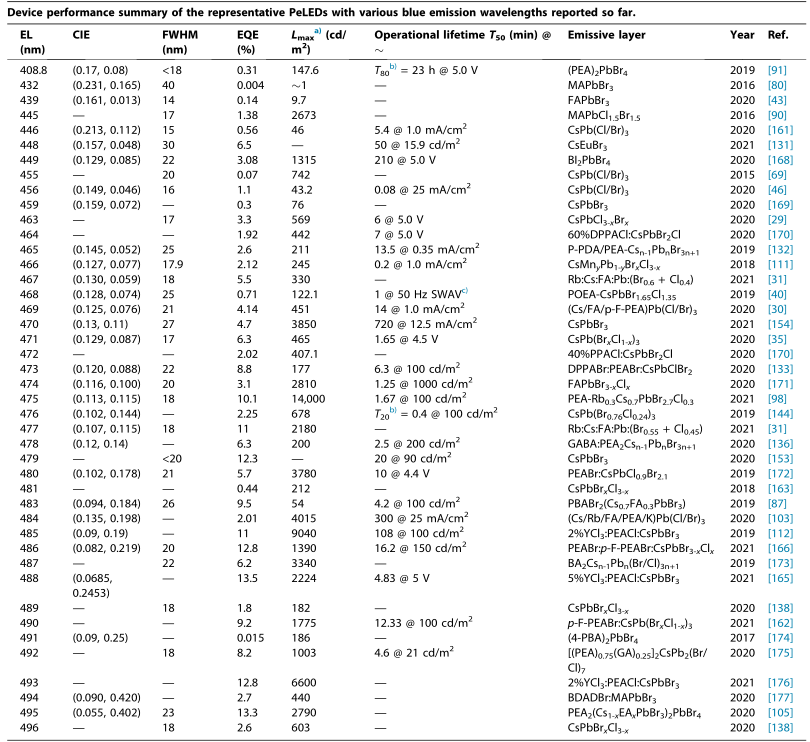
\includegraphics[width=.8\linewidth]{pic/10.png}
        \caption{近年来不同蓝光PeLED的性能\cite{zhang2021blue}}
	\end{figure}
\par 为了使蓝PeLED的发射波长调整到真蓝范围(455nm-470nm),要么需要过量的Cl$^-$取代Br$^-$,要么需要减小钙钛矿量子点的尺寸以获得更高的激子束缚能。然而通过本文2.1节的内容可知Cl$^-$越多合成的混合卤素钙钛矿膜含有更多的缺陷,并且长链配体的存在虽然减小了钙钛矿量子点的尺寸,但是也会阻碍了电荷载体的注入和输运,导致钙钛矿薄膜的导电性较差。
\subsubsection{光谱稳定性问题}
\par 由于钙钛矿材料具有较低的晶格形成能\cite{pan2019halogen},容易产生离子缺陷,因此在基于钙钛矿结构的光电器件中,离子迁移是一个值得关注的问题。在热、化学梯度、光激发、电场等外部输入下,形成能较低的卤素离子会沿空位缺陷特别是晶界区域迁移,离子迁移导致混合卤化物PeLED的光谱不稳定(即颜色不稳定)和钙钛矿太阳能电池的迟滞效应\cite{xiao2017efficient}。由于卤化物的分离,光谱稳定性是实现稳定的蓝光发射PeLED的重要挑战之一。
\par 制备混合阳离子钙钛矿是稳定混合卤化物球团发射光谱的有效方法,这是混合阳离子可以使得晶格形成能的增加,从而减少空位缺陷的形成,因此我们可以通过一种具有较小离子半径的替代二价金属元素来减少钙钛矿中卤素空位缺陷的形成。
\par 为实现具有高效蓝光发射和良好光谱稳定性的PeLED,我们也可以考虑配体作用的影响,在钙钛矿前驱体溶液中引入不同的配体可以影响其结晶过程,从而调节蓝色发射波长,并通过操纵堆积的体积大的有机配体之间的范德瓦尔斯相互作用来提高光谱稳定性。
\subsubsection{Pb元素的毒性}
\par Pb元素的毒性是PeLED商业化应用面临的另一个挑战。含铅体系相对稳定,降解时间较长,会对环境造成破坏。因此,有必要用其他低毒性或无毒的金属元素替代铅。Sn$^{2+}$与Pb$^{2+}$在半径等许多方面具有相似之处,是Pb$^{2+}$的理想替代品,但Sn$^{2+}$在空气中容易被氧化为Sn$^{4+}$,从而产生不良的高自由载流子密度,导致钙钛矿膜PL猝灭。与Sn$^{2+}$相比,Bi$^{3+}$和Sb$^{3+}$在空气中更稳定,但是铋卤化物和锑卤化物不能形成三维框架。
\par 另一种类型的无铅蓝MHP是卤化物双钙钛矿结构(A$_2$BB$^{\prime}$X$_{6}$),其中单价B(例如Cu$^{+}$,Au$^{+}$等)和一个三价B$^{\prime}$(例如Sb$^{3+}$或Bi$^{3+}$)离子结合以实现总体电荷平衡,然而卤化物双钙钛矿是间接带隙半导体,具有宽PL光谱,因此不能用作电致发光器件的发射器,也不适合用于超高清显示应用。
\subsection{如何提高蓝光PeLED效率}
\subsubsection{A位离子掺杂}
\par 离子掺杂可以有效地修饰钙钛矿材料的结构、光学和电子性能,目前在钙钛矿材料的制备中已被广泛应用。钙钛矿材料的混合A位点阳离子策略可以提高钙钛矿太阳能电池的效率和稳定性,同样,钙钛矿交替的A位组成也可以提高PeLED的性能。少量的有机阳离子引入CsPbBr$_{3}$增加了钙钛矿的PL发射由于Pb抑制的金属复合中心,确认Cs的引入有利于蓝色PeLED的长期稳定。
	\begin{figure}[H]
		\centering
		\hspace{2em}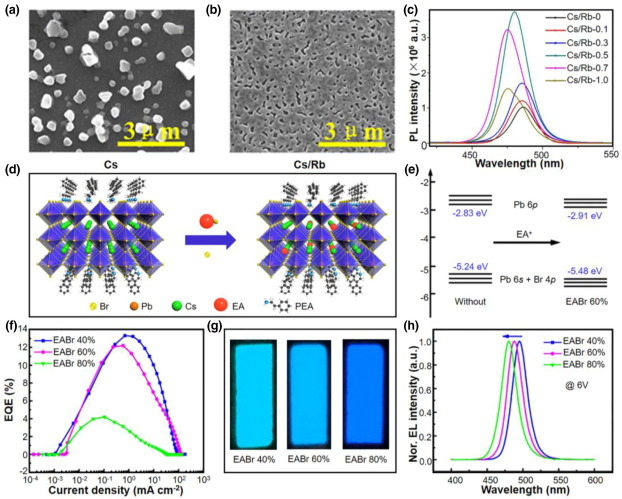
\includegraphics[width=.8\linewidth]{pic/8.jpg}
		\caption{(a)(b)不掺杂与掺杂薄膜的形态(c)掺杂Rb不同浓度的PL谱(d)(e)掺杂Rb后的晶体结构与能带结构,(f)(g)(h)A位离子掺杂EA后光谱表征\cite{zhang2021blue}
		}
	\end{figure}
\par 铷(Rb)是制备蓝光发射钙钛矿材料中最常用的A位阳离子掺杂剂,其半径比Cs小。由于钙钛矿结构的灵活性,通过改变A位阳离子的大小,我们将原子视为刚性小球模型可知,不同的离子半径可以对角共八面体骨架施加化学压力\footnote{这也是典型钙钛矿结构容错因子的由来,如果不满足容错因子的范围就会产生八面体结构的断裂,也就不是钙钛矿结构了。},这会导致结构的扭曲,如八面体的倾斜和八面体阳离子偏离中心的位移,从而改变Pb$^{2+}$与卤素离子之间的反键轨道重叠。当Rb$^+$掺杂到钙钛矿晶格中时,Pb$^{2+}$与卤素离子反键轨道重叠减小,从而增大了钙钛矿的带隙。因此,钙钛矿与Rb$^+$的掺杂可以调节PL发射向更短的波长。同时Rb$^+$的引入可以改善CsPb(Cl/Br)$_3$钙钛矿薄膜的形貌和光学性能(如图9b)。
\par 同样的我们可以通过增加半径大的有机阳离子减少Pb-Br轨道耦合并增加蓝色发射的带隙(如图9e),同样的这样的掺杂可以改善PeLED的光学性能与蓝光发射(如图9f-h)。
\subsubsection{B位离子掺杂}
\par 根据上一小节对A位离子掺杂的内容,我们知道这是由于八面体结构产生变化导致的电子云轨道重叠发生变化,从而改善蓝光发射波长,同样的,我们也可以通过B位离子的掺杂达到相同的效果,而且由于位于共角八面体中心的B位元素不仅通过改变八面体旋转或倾斜的程度影响钙钛矿的晶相,而且还决定了它们的电子能带结构,因此不同金属离子部分取代Pb$^{2+}$是调节钙钛矿材料发射波长,提高其稳定性和光电性能的一种可能方法。
	\begin{figure}[H]
		\centering
		\hspace{2em}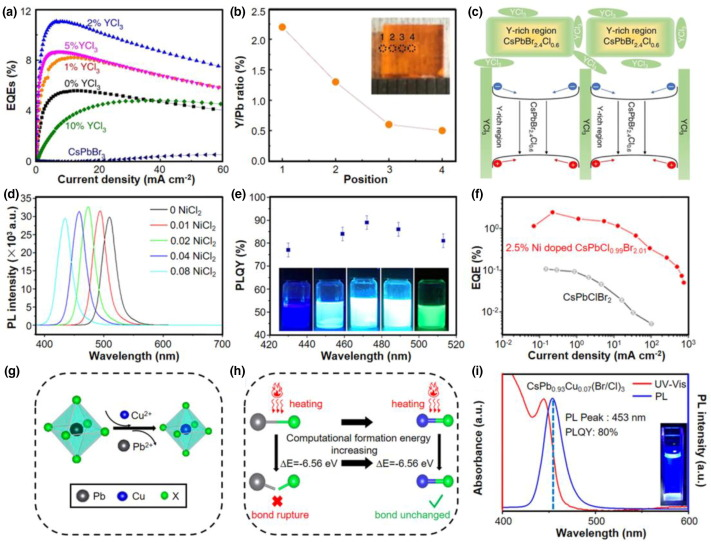
\includegraphics[width=.8\linewidth]{pic/9.jpg}
		\caption{(a)不同YCl$_{3}$配比下PeLED的EQE曲线;(b) CsPbBr$_{3}$钙钛矿晶体不同位置的Y/Pb比值;(c)薄膜中Y$^{3+}$的梯度分布及其对颗粒中载流子的限制作用示意图;(d)(e)(f)不同掺杂Ni$^{2+}$下参数的表征;(g)(h)(i)掺杂Cu$^{2+}$下的光谱参数表征
        \cite{zhang2021blue}
		}
	\end{figure}
\par 我们由图10a可以看出掺杂适量的Y可以改善蓝光发射并提高器件的EQE,而且添加的YCl$_3$不仅掺杂到钙钛矿晶格中(如图10b),还存在于晶界和晶面,有效地限制了晶内的载流子,有利于辐射重组(如图10c)。
\par 此外,Ni$^{2+}$掺杂可以有效消除卤化物空位等固有缺陷,并导致晶格的近程序增加。通过密度泛函理论计算可以证明了Ni掺杂导致了缺陷形成能的增加,而没有在带隙中引入深阱态,可以导致局部结构有序改善和PLQY显著增强(如图10d-f),同样的,Cu$^{2+}$掺杂也能起到和Ni$^{2+}$掺杂同样的效果(如图10g-i)。
\subsubsection{表面配体的作用}
\par 在胶体钙钛矿量子点的合成中,表面配体可以保持颗粒在溶液中的单分散性,钝化钙钛矿的表面缺陷,提高材料的稳定性。油酸(OA)和油胺(OAm)是合成钙钛矿常用的两种表面配体,其中油胺的油胺离子(OAm$^+$)取代CsPbBr$_3$表面的Cs$^+$作为盖层配体。而油酸并不结合在钙钛矿纳米晶的表面,只是反应混合物中的残余部分,以维持纳米晶的胶体稳定性。其中,油酸可以抑制钙钛矿纳米碳化物的团聚,提高其稳定性;油胺可以通过影响晶化动力学来防止钙钛矿纳米碳化物形成大晶粒。然而这些配体在钙钛矿上表现出高度动态和松散的结合,在隔离和纯化过程中很容易从表面脱落,导致钙钛矿样品的降解。为了使钙钛矿样品具有理想的稳定性和光学特性,需要保持这些组分之间的平衡。
\par 根据本文3.1节的内容我们知道,钙钛矿发光层中载流子的有效注入和传输是实现高效PeLED的前提之一。胶体钙钛矿量子点通常被配体分子包裹,然而这些碳氢化合物长链具有电子绝缘性,阻碍了电荷载流子注入PeLED中的钙钛矿发光层。为了解决这一问题,很容易想到的是我们需要减少有机配体的数量,或者用更短的配体取代这些长配体,但很可惜的是就目前我查找文献的结果来看,在减少配体或者用短链配体取代方面的研究很少或者说结果不显著。
\par 不过目前有文献介绍为了优化有机配体的数量,我们可以采用了一种三辛基氧化膦(TOPO)介导的一步方法\cite{peng2020effective},通过改变TOPO的数量,有效地调节钙钛矿表面配体的浓度。这是因为TOPO可以很容易地与游离油酸中的酸性质子结合,形成脱质子油酸基的酸碱络合物,而脱质子油酸基可以很容易地通过纯化去除。此外,TOPO-PbBr$_2$的形成可以减少欠配位Pb$^{2+}$\footnote{由于我本研也是做的钙钛矿量子点相关的工作,也尝试过添加TOPO介导的方法,但是就结果而言似乎对于量子点缺陷的钝化效果提升都不明显。}。
\par 还有另一种增强载体注入和转运以及改善胶体钙钛矿发光特性的有效方法是通过引入高迁移率的无机配体来部分替代有机配体,从而提高薄膜的电导率和辐射重组。通过引入碱金属K$^{+}$作为一种新型配体,并通过减少绝缘有机配体可以得到了具有优越电导率的钙钛矿薄膜\cite{yang2020efficient}。同时发现利用PrCl$_{3}$对PeLED进行了预优化,不仅可以有效地钝化表面的Cl空位,还可以通过取代它们来适当地减少它们表面的长链有机配体。
\clearpage
\section{总结与展望}
\par PeLED有着高光致发光量子子产率、低陷阱态密度、高颜色纯度和宽色域等优点,我们分析了PeLED的结构,并且讨论得出在与传统OLED和QLED的对比中占有很大的优势,而且PeLED在近几年的研究中取得了很大的进步,尤其是绿光和红光PeLED的EQE已经正在赶上OLED和QLED。但是,高效的蓝光PeLED仍然是一个挑战,同时对于PeLED而言,光谱稳定性、离子迁移以及迟滞效应也是很大的一个问题。
\par 在这次的pre以及课程论文中我着重讨论了蓝光PeLED所面临的主要挑战以及目前的一些解决办法。目前满足超高清电视标准的真蓝区域(455$\sim$470nm)发射波长的蓝色PeLED的效率仍然很低,这是未来需要解决的关键问题。同时,老师在课堂上提出的关于PeLED器件结构相关的问题与讨论,在提升PeLED器件EQE方面,我们也可以从器件本身的结构入手思考通过器件结构的设计来提高出光效率,这可能也会是以后PeLED走向市场前需要关注的问题。同时虽然混合卤化物策略确实可以很方便地获得真蓝钙钛矿发射体,但这种类型的钙钛矿经常发生不同卤素相之间的分离。通过添加掺杂剂和添加剂、调整材料组成等方法我们可以优化钙钛矿薄膜,以更好地稳定具有离子性质的蓝色钙钛矿。当然,表面有机配体还会阻碍空穴电子载流子的传输,如何优化配体组成也是一个问题。同样的,Pb的毒性是未来研究中需要解决的另一个问题,我们还需要探索新型无铅钙钛矿。尽管PeLED目前还是存在着很大的问题,但是相较于钙钛矿材料的相对这么好的优势,我相信在不久的将来,PeLED一定会走向商用化的道路。
\clearpage
\section{致谢与课程建议}
\par 感谢一学期以来陈志忠教授对于宽禁带半导体内容的精彩讲授以及邓楚涵助教在课后对于我个人一些疑惑的解答,让我学到了很多关于宽禁带半导体器件方面实用化的知识技能,以及感谢在课程演讲部分各位同学的精彩演讲,各位同学的报告内容涉及非常广泛让我拓宽了视野,尽管我现在对于报告的大部分方向都没有涉及无法提出高质量有效的问题,但是同学们的报告也让我受益匪浅。
\par 陈志忠教授在本学期讲授的宽禁带半导体课程先是介绍了一些基本的宽禁带半导体材料及其应用与特点,接着主要讲授了GaN,InGaN和AlGaN此类宽禁带半导体材料的制备方法,最后讲述了一些器件结构的制作以及如何提高器件效率与出光效率的方法。总体而言通过本课程的学习能够达到一个快速入门宽禁带半导体的效果,但是可能是由于课程时间的紧张,导致个人认为在器件方面的讲述内容偏少,个人认为相比于材料外延生长制备方法而言,可以稍多介绍一些宽禁带半导体在光电探测,太阳能电池以及纳米激光器等器件方面具体的应用,以及虽然GaN是本课程介绍的重点,其中也希望可以多穿插一些新兴半导体或者低维半导体材料的介绍,这样也能更好体现出课程的前沿性。
\par 最后,希望宽禁带半导体这门课越开越好,选课人数越来越多!
\clearpage
\printbibliography[heading=bibintoc]
\end{document}